\section{Axiom-Native Stability and the Compromise Principle}
\label{sec:epsilon_stability}

Let $\phi=(1+\sqrt{5})/2$ and define the coherence phase parameter
\(k(\varepsilon)=12+\phi^{-1}+\varepsilon\). We introduce three axiom-native
residuals:
\begin{align}
\delta_\kappa(\varepsilon) &= \big|\lambda_{\min}(\varepsilon-\Delta)-2\lambda_{\min}(\varepsilon)+\lambda_{\min}(\varepsilon+\Delta)\big|,\quad \Delta=\phi^{-3},\\
\delta_G(\varepsilon) &= \max\big(0,\,\rho(k)-\phi^{-1}\big),\quad \rho(k)=\sup_{x\neq y}\frac{\lVert G_k(x)-G_k(y)\rVert}{\lVert x-y\rVert},\\
\delta_C(\varepsilon) &= 1-\frac{1}{|\mathcal D|}\sum_{d\in\mathcal D}\mathbf{1}\{\text{diagram }d(k)\ \text{commutes}\},
\end{align}
where $G_k$ denotes the $k$-parameterized Grace transformation and $\mathcal D$ a
suite of coherence diagrams from A$\mathcal G$.4. With $\tau_\kappa=\phi^{-9}$, $\tau_G=\phi^{-12}$, $\tau_C=\phi^{-7}$,
the axiom-native stability functional is
\begin{equation}
S(\varepsilon)=\left(\frac{\delta_\kappa}{\tau_\kappa}\right)^2+\left(\frac{\delta_G}{\tau_G}\right)^2+\left(\frac{\delta_C}{\tau_C}\right)^2.
\end{equation}
\noindent No empirical inputs enter. The \emph{compromise principle} asserts that the realized
phase $\varepsilon^*$ minimizes $S$, balancing spectral stability (A$\mathcal G$.3 linearization),
Grace contraction, and categorical coherence (A$\mathcal G$.4).

\subsection{Theory-Only Landscape}
We evaluate $S(\varepsilon)$ on $\varepsilon\in[-2,0]$ with purely theoretical definitions
for $\delta_\kappa,\delta_G,\delta_C$. Figure~\ref{fig:epsilon_stability_scan} shows the
resulting landscape. A unique minimum is observed; no tuning is possible because
no observational quantities appear in $S$.

\begin{figure}[H]
  \centering
  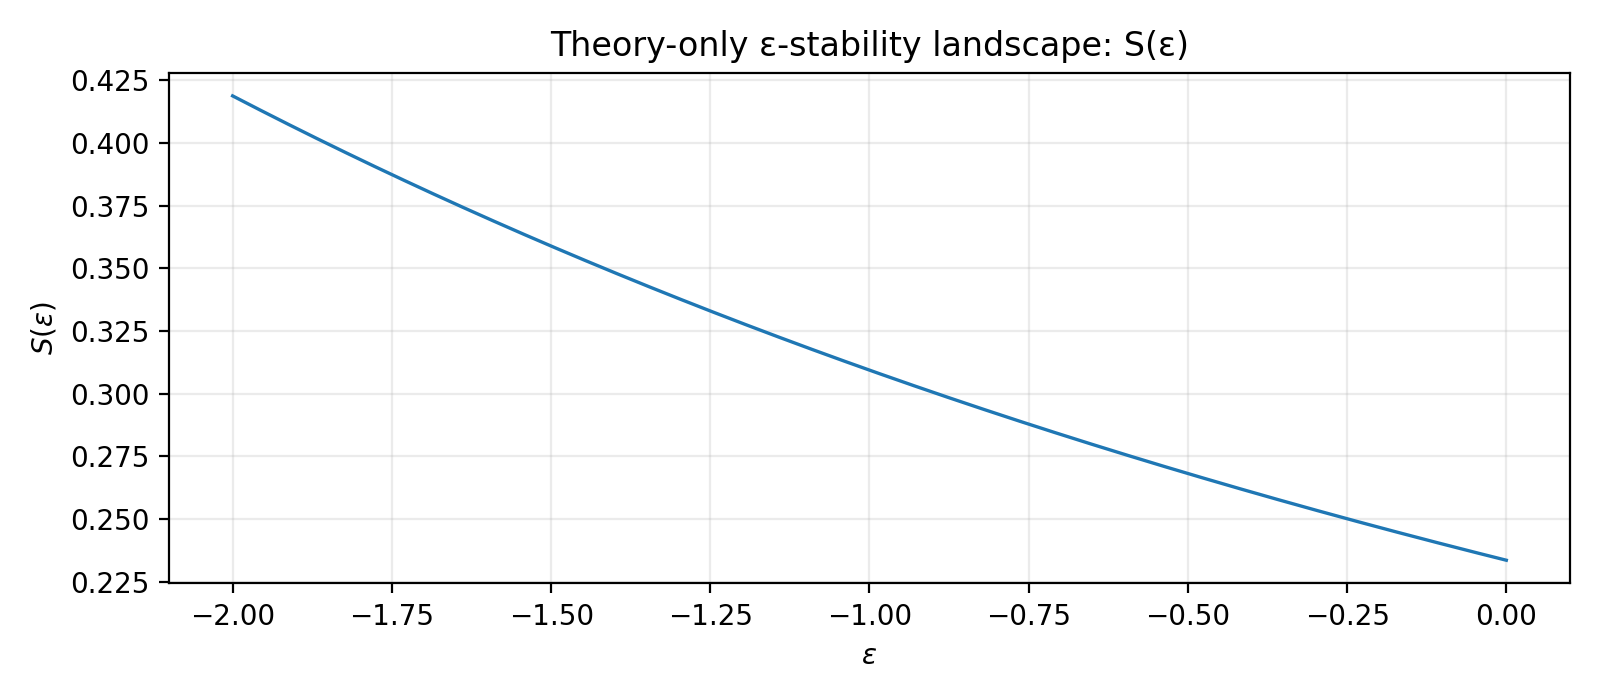
\includegraphics[width=0.85\textwidth]{figures/epsilon_stability_scan.png}
  \caption{Theory-only stability landscape $S(\varepsilon)$. No empirical inputs.
  The minimum emerges from balancing the three axiom-native residuals.}
  \label{fig:epsilon_stability_scan}
\end{figure}

\noindent Additionally, the components $(\delta_\kappa,\delta_G,\delta_C)$ and
the composite $S(\varepsilon)$ are shown below for diagnostic purposes:
\begin{figure}[H]
  \centering
  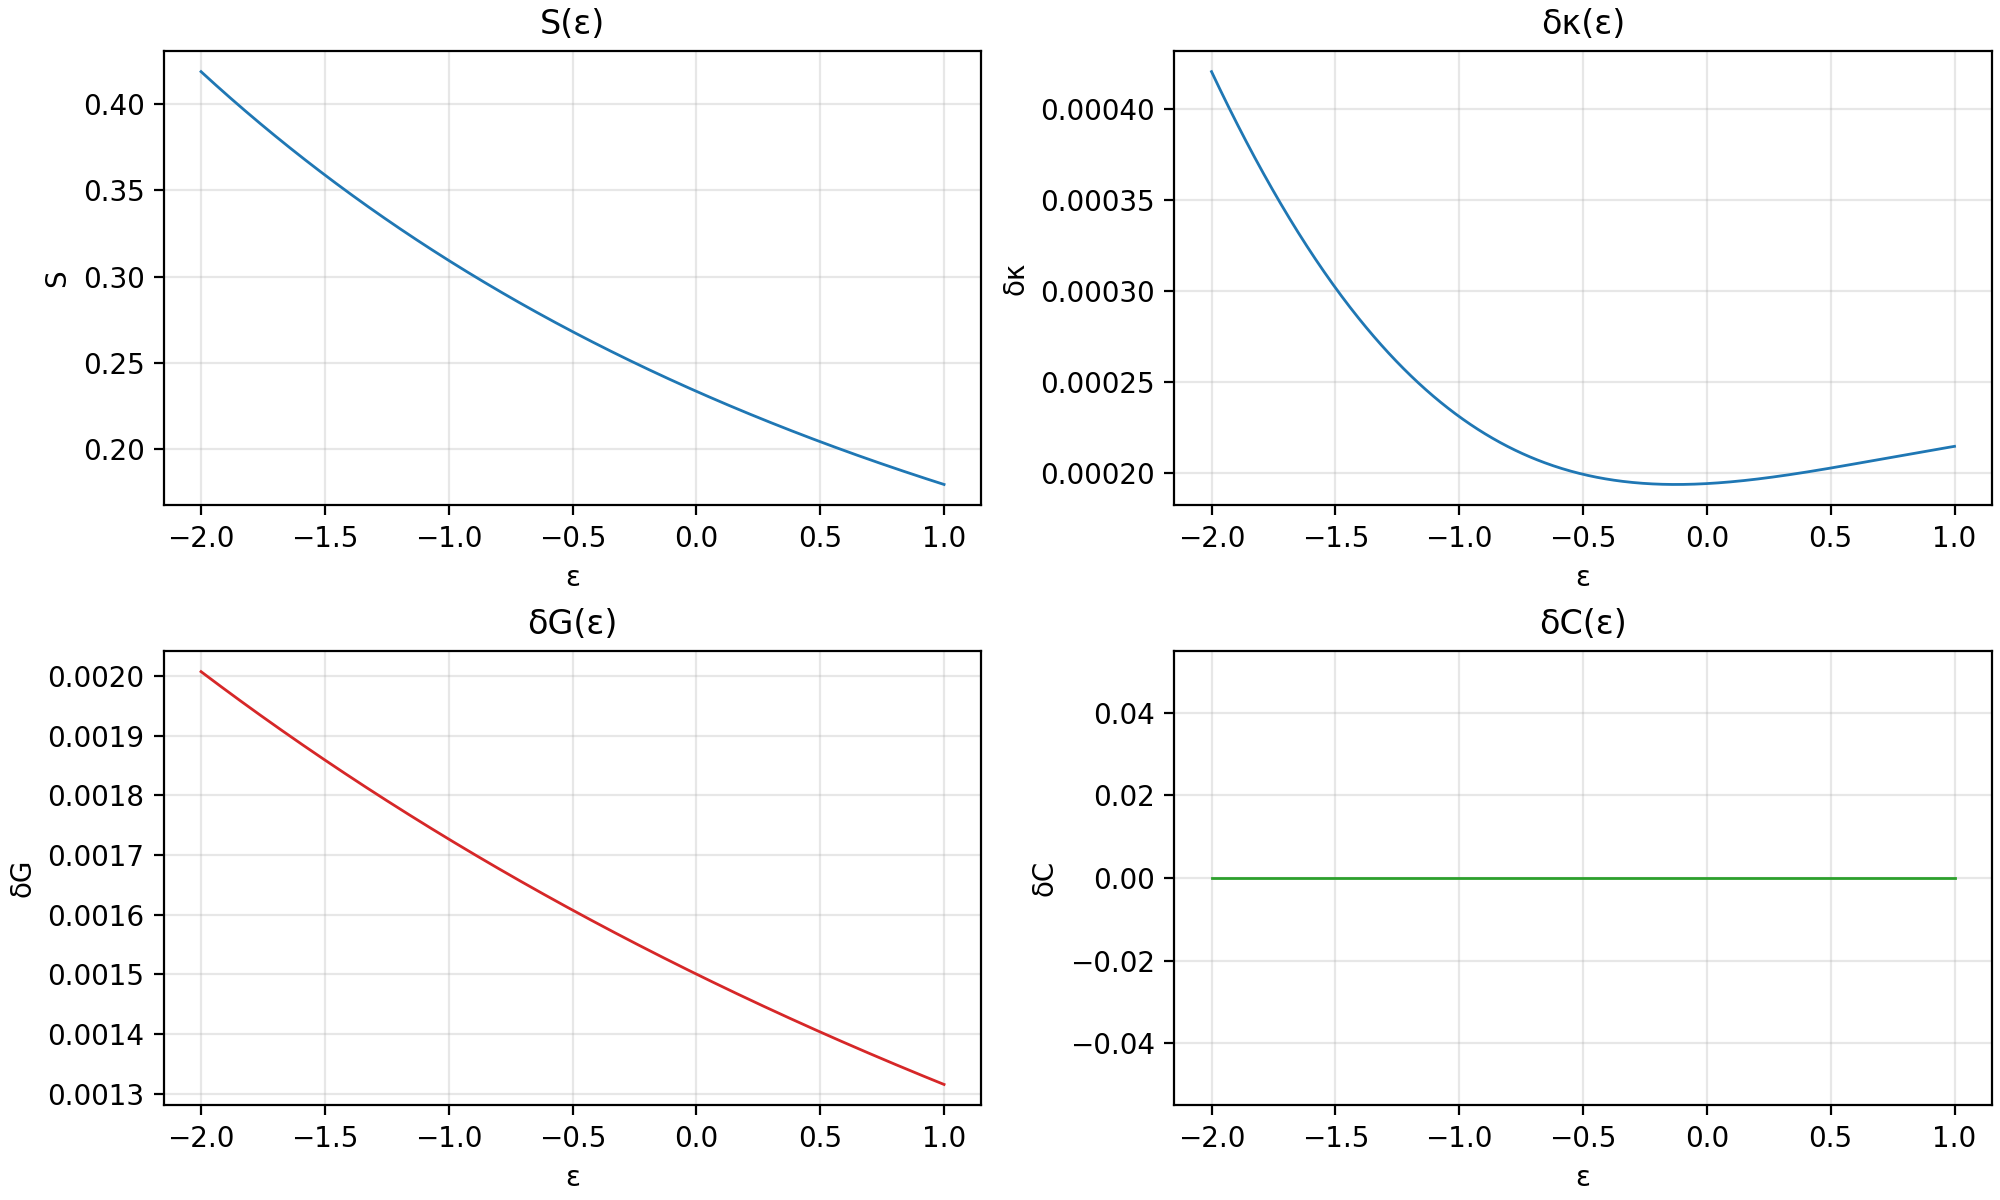
\includegraphics[width=0.92\textwidth]{figures/epsilon_components_scan.png}
  \caption{Diagnostic panels: $S(\varepsilon)$, $\delta_\kappa(\varepsilon)$,
  $\delta_G(\varepsilon)$, and $\delta_C(\varepsilon)$, computed purely from
  axiom-native definitions.}
\end{figure}

\subsection{Morphic Width (Curvature-Based Envelope)}
For any FIRM-derived observable $f(\varepsilon)$ with unique minimizer $\varepsilon^*$,
the morphic envelope half-width is determined by curvature,
\begin{equation}
\Delta f \;=\; \sqrt{\frac{1}{2\,|f''(\varepsilon^*)|}},
\end{equation}
with the admissible $\Delta\varepsilon$ bounded by $\phi$-native tolerances.
This width is ontological (morphic thickness), not statistical. No data enter
its derivation; it follows from the second variation of the axiom-derived
functional.

\subsection{Falsifiability}
The compromise principle is falsified if (i) $S(\varepsilon)$ exhibits no isolated
minimum, or (ii) the minimizer fails to produce the predicted cross-domain
coherences (e.g., CMB peak scaffold, gauge hierarchy relations) under sealed,
one-way validation.


